\documentclass[border=4pt]{standalone}
\usepackage{tikz}
\usepackage{amssymb}
\usepackage{amsmath}
\usetikzlibrary{arrows.meta}
\definecolor{waveblue}{HTML}{3A7CA5}
\definecolor{wavered}{HTML}{D1495B}
\definecolor{mazewall}{HTML}{2B2B2B}

% shared 6x6 perfect maze (a spanning tree over the grid): exactly one
% simple route from S to G: every other branch is a genuine dead end.
\newcommand{\mazewalls}{
  \draw[mazewall, line width=2pt] (0,0) rectangle (6,6);
  \draw[mazewall, line width=1.6pt] (0,1) -- (1,1);
  \draw[mazewall, line width=1.6pt] (2,0) -- (2,1);
  \draw[mazewall, line width=1.6pt] (5,0) -- (5,1);
  \draw[mazewall, line width=1.6pt] (1,2) -- (2,2);
  \draw[mazewall, line width=1.6pt] (2,1) -- (2,2);
  \draw[mazewall, line width=1.6pt] (2,2) -- (3,2);
  \draw[mazewall, line width=1.6pt] (3,1) -- (3,2);
  \draw[mazewall, line width=1.6pt] (4,1) -- (4,2);
  \draw[mazewall, line width=1.6pt] (4,2) -- (5,2);
  \draw[mazewall, line width=1.6pt] (5,2) -- (6,2);
  \draw[mazewall, line width=1.6pt] (0,3) -- (1,3);
  \draw[mazewall, line width=1.6pt] (1,3) -- (2,3);
  \draw[mazewall, line width=1.6pt] (3,2) -- (3,3);
  \draw[mazewall, line width=1.6pt] (3,3) -- (4,3);
  \draw[mazewall, line width=1.6pt] (4,3) -- (5,3);
  \draw[mazewall, line width=1.6pt] (1,4) -- (2,4);
  \draw[mazewall, line width=1.6pt] (2,3) -- (2,4);
  \draw[mazewall, line width=1.6pt] (3,3) -- (3,4);
  \draw[mazewall, line width=1.6pt] (5,3) -- (5,4);
  \draw[mazewall, line width=1.6pt] (2,4) -- (2,5);
  \draw[mazewall, line width=1.6pt] (3,4) -- (3,5);
  \draw[mazewall, line width=1.6pt] (4,4) -- (4,5);
  \draw[mazewall, line width=1.6pt] (4,5) -- (5,5);
  \draw[mazewall, line width=1.6pt] (1,5) -- (1,6);
  \draw[mazewall, line width=1.6pt] (4,5) -- (4,6);
}
% the one true S->G solution route
\newcommand{\solutionpath}{
  (0.5,0.5) -- (1.5,0.5) -- (1.5,1.5) -- (0.5,1.5) -- (0.5,2.5) -- (1.5,2.5) -- (2.5,2.5) -- (2.5,3.5) -- (2.5,4.5) -- (2.5,5.5) -- (3.5,5.5) -- (3.5,4.5) -- (3.5,3.5) -- (4.5,3.5) -- (4.5,4.5) -- (5.5,4.5) -- (5.5,5.5)
}
% two genuine dead-end branches (walked, then must backtrack)
\newcommand{\deadendA}{
  (5.5,0.5) -- (5.5,1.5) -- (4.5,1.5) -- (4.5,0.5) -- (3.5,0.5) -- (3.5,1.5) -- (3.5,2.5) -- (4.5,2.5) -- (5.5,2.5) -- (5.5,3.5) -- (5.5,4.5)
}
\newcommand{\deadendB}{
  (1.5,3.5) -- (0.5,3.5) -- (0.5,4.5) -- (1.5,4.5) -- (1.5,5.5) -- (2.5,5.5)
}

\begin{document}
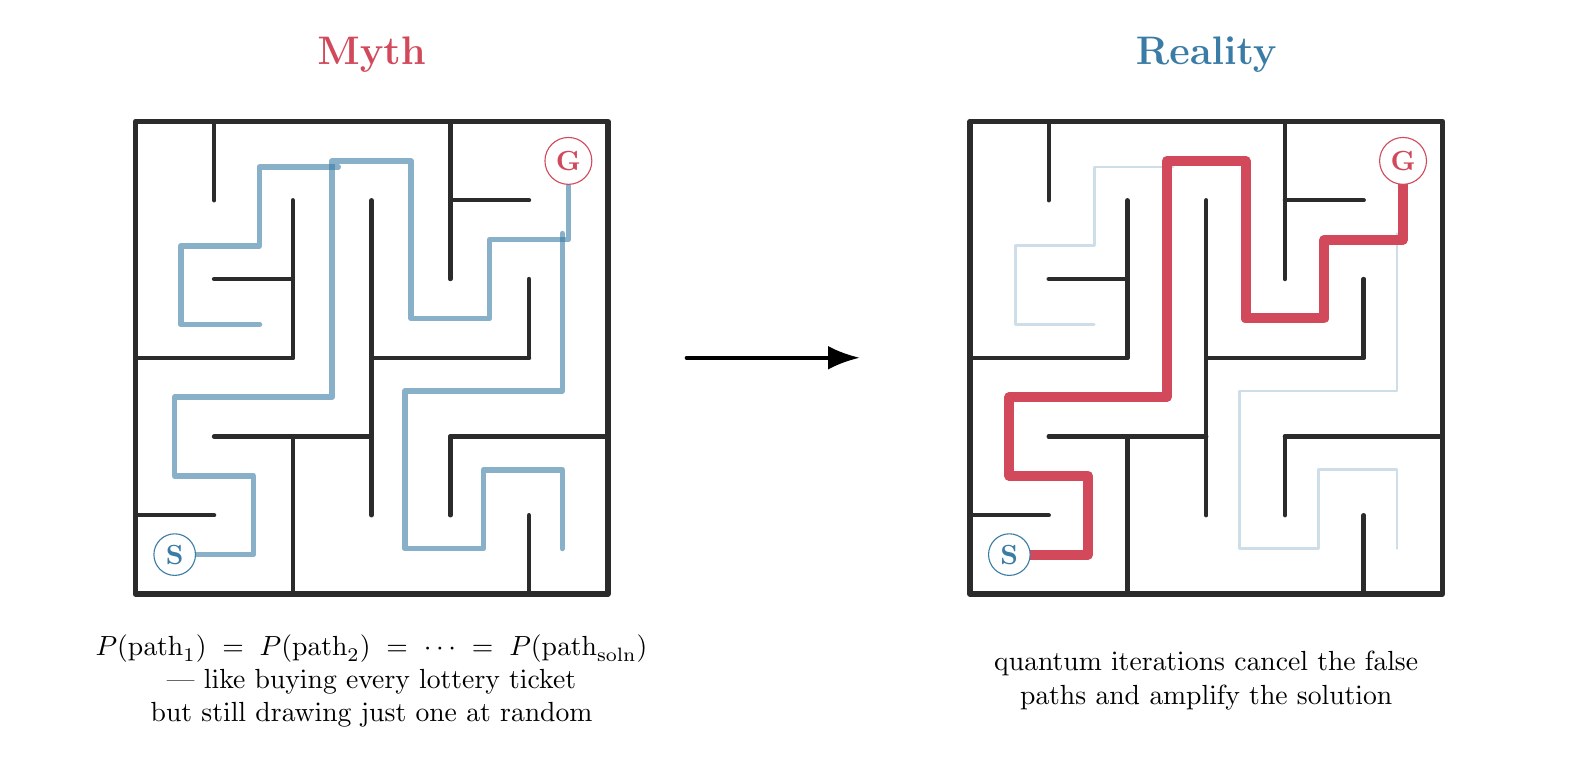
\begin{tikzpicture}[line cap=round, line join=round]

  % ============ Left panel: "the myth" ============
  \begin{scope}[shift={(0,0)}]
    \node[wavered, font=\Large\bfseries] at (3,6.85) {Myth};

    \mazewalls

    % all branches -- dead ends and the one true path -- explored with
    % equal amplitude; offset each slightly so the equal superposition
    % of distinguishable paths is visible rather than overlapping
    \draw[waveblue, line width=2pt, opacity=0.6, xshift=-2.2pt, yshift=2.2pt] \deadendA;
    \draw[waveblue, line width=2pt, opacity=0.6, xshift=2.2pt, yshift=-2.2pt] \deadendB;
    \draw[waveblue, line width=2pt, opacity=0.6] \solutionpath;

    \node[waveblue, font=\bfseries] at (0.5,0.5) [circle, fill=white, draw=waveblue, inner sep=2pt] {S};
    \node[wavered, font=\bfseries] at (5.5,5.5) [circle, fill=white, draw=wavered, inner sep=2pt] {G};

    \node[font=\normalsize, align=center, text width=8.5cm] at (3,-1.1)
      {$P(\text{path}_1)=P(\text{path}_2)=\cdots=P(\text{path}_{\text{soln}})$\\ --- like buying every lottery ticket but still drawing just one at random};
  \end{scope}

  % ============ Divider ============
  \draw[-{Latex[length=4mm]}, line width=1.3pt] (7.0,3) -- (9.2,3);

  % ============ Right panel: "the reality" ============
  \begin{scope}[shift={(10.6,0)}]
    \node[waveblue, font=\Large\bfseries] at (3,6.85) {Reality};

    \mazewalls

    % dead ends now faint/shrunk -- their amplitude has been suppressed
    \draw[waveblue, line width=1pt, opacity=0.25, xshift=-2.2pt, yshift=2.2pt] \deadendA;
    \draw[waveblue, line width=1pt, opacity=0.25, xshift=2.2pt, yshift=-2.2pt] \deadendB;

    % the one true solution, amplified after r rounds of oracle + diffuser
    \draw[wavered, line width=3.6pt] \solutionpath;

    \node[waveblue, font=\bfseries] at (0.5,0.5) [circle, fill=white, draw=waveblue, inner sep=2pt] {S};
    \node[wavered, font=\bfseries] at (5.5,5.5) [circle, fill=white, draw=wavered, inner sep=2pt] {G};

    \node[font=\normalsize, align=center, text width=8.5cm] at (3,-1.1)
      {quantum iterations cancel the false paths and amplify the solution};
  \end{scope}

\end{tikzpicture}
\end{document}
